\chapter{Projeto - Parte 2}\label{ch:projeto-parte2}

Nesta fase do projeto, o objetivo foi criar um sistema inteligente capaz de se movimentar num espaço bidimensional com dimensões fixas onde existem obstáculos.
A finalidade do agente prospetor é recolher os alvos e evitar os obstáculos presentes no ambiente (ver figura~\ref{fig:agente-prospetor}).
O agente pode ser considerado homólogo a um robô móvel autónomo (e.g., um robô que aspira sozinho a casa), que se pode mover nos quatro sentidos cardeais (i.e., norte, sul, este e oeste).

\begin{figure}[H]
    \begin{center}
        \resizebox{100mm}{!}{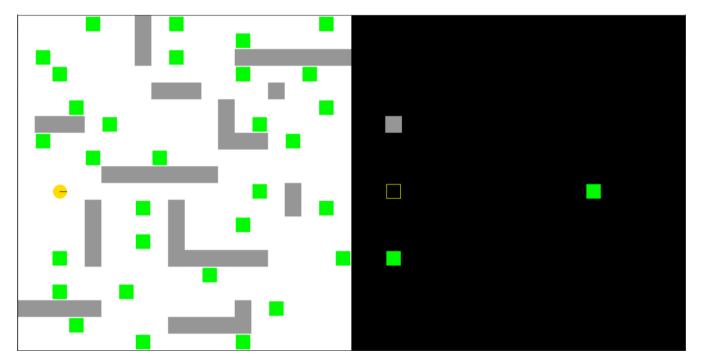
\includegraphics{../figures/agente-prospetor}}
    \end{center}
    \caption{Representação visual desta fase do projeto.
    Retirado de~\cite{isel:iasa:slides:arq-agentes-reativos-parte-2}, slide 13.}\label{fig:agente-prospetor}
\end{figure}

Para que o agente possa atingir os objetivos propostos, foi necessário implementar um agente reativo e os seus módulos comportamentais associados.
O agente reativo foi implementado com base na biblioteca ECR (Esquemas Comportamentais Reativos) criada para esta fase do projeto, que expõe os mecanismos base de comportamento (e.g., reação, estímulo, resposta).
A interação com o ambiente foi realizada através da biblioteca SAE (Simulador de Ambiente de Execução),
que foi disponibilizada para esta fase do projeto.

Tal como em fases anteriores, a implementação foi feita com base na consulta e compressão de diagramas UML e de sequência de forma a garantir a correta implementação dos diferentes subsistemas.


\section{Agentes Reativos}\label{sec:agentes-reativos}

Na secção da arquitetura de agentes (ver secção~\ref{sec:arquiteturas-agente}), foi referido que uma arquitetura reativa é caracterizada pela associação direta entre perceções e ações.
Associada a esta arquitetura está a ideia de que um agente reativo é composto por um conjunto de reações, e que são organizadas de forma modular em módulos comportamentais designados por comportamentos.

\subsection{Reação}\label{subsec:reacao}

Inerente à arquitetura de agentes reativos, está o conceito de mecanismo de reação e que apresenta os seguintes elementos:

\begin{itemize}
    \item \textbf{Estímulo}: Define a informação que é extraída de uma perceção, de forma a ser utilizada na ativação de uma resposta.
    Vários estímulos podem ser ativados por uma única perceção.
    Estão regularmente associados a um parâmetro de intensidade, que pode ser utilizado para determinar a prioridade de ativação de uma resposta;
    \item \textbf{Resposta}: Representa a geração de uma resposta a estímulos, inerentemente ligada a uma ação a ser executada e à sua respetiva prioridade.
    Além de poder ser ativada por um estímulo, uma resposta pode ser ativada diretamente por uma perceção, de forma a garantir restrições de ativação (i.e., guardas) se necessário;
    \item \textbf{Reação}: Módulo que associa estímulos a respostas.
\end{itemize}

Um agente reativo é composto por um conjunto de reações, que devem ser organizadas de forma modular em módulos comportamentais designados por comportamentos.
Isto permite que as reações internas do agente sejam encapsuladas, facilitando a sua manutenção e escalabilidade.

\subsection{Comportamento}\label{subsec:comportamento}

Um comportamento (ver figura~\ref{fig:agente-reativo-comportamento}) define um módulo associado ao processamento de perceções do módulo de controlo de um agente reativo, onde é definida a forma como os objetivos implícitos do agente devem ser concretizados. Encapsula um conjunto de reações relacionadas entre si, possivelmente com uma sequência temporal, de forma a atingir um ou mais objetivos (e.g., evitar obstáculos, recolher alvos, etc). Associado a um objetivo podem existir sub-objetivos.

\begin{figure}[H]
    \begin{center}
        \resizebox{100mm}{!}{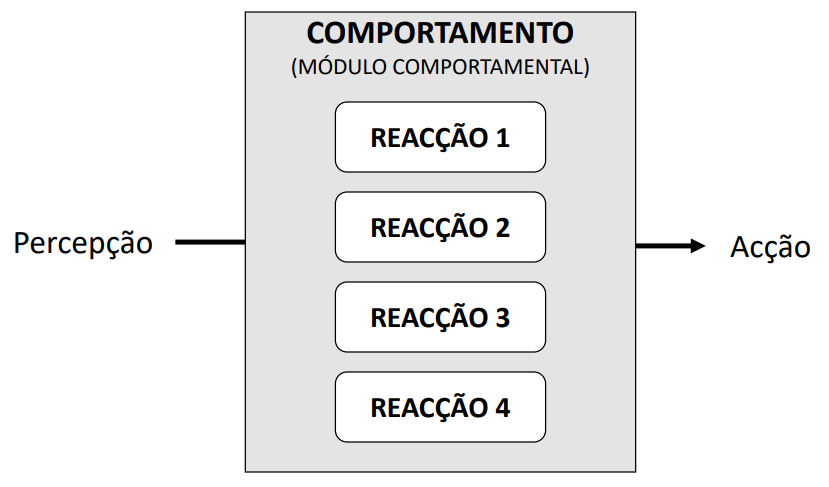
\includegraphics{../figures/agente-reativo-comportamento}}
    \end{center}
    \caption{Módulo comportamental de um agente reativo.
    Retirado de~\cite{isel:iasa:slides:arq-agentes-reativos-parte-1}, slide 11.}\label{fig:agente-reativo-comportamento}
\end{figure}

Tipos de Comportamento:

\begin{itemize}
    \item \textbf{Comportamento Fixo}: Caracterizado por ter uma resposta fixa, pois gera uma ação em permanência;
    \item \textbf{Comportamento Simples}: Reação;
    \item \textbf{Comportamento Composto}: Agrega sub-comportamentos, ao qual está associado um mecanismo de seleção de ação de forma a determinar a ação a realizar em função das respostas dos mesmos.
\end{itemize}

\subsection{Comportamento Composto}\label{subsec:comportamento-composto}

Como em comportamentos compostos, uma perceção pode ativar múltiplas reações, as quais geram diferentes ações, é necessário definir um mecanismo de seleção de ação.
Alguns dos mecanismos de seleção de ação mais comuns são:

\begin{itemize}
    \item \textbf{Execução paralela}: As ações são executadas em paralelo, porque não interferem entre si;
    \item \textbf{Seleção por prioridade}: As ações são selecionadas em função de uma prioridade.
    É possível distinguir dois tipos de comportamentos compostos com seleção por prioridade:
    \begin{itemize}
        \item \textbf{Prioridade}: Representa uma forma de comportamento composto com um mecanismo de seleção de ação de prioridade dinâmica, e que portanto a prioridade dos comportamentos associados varia consoante o tempo (e.g., o comportamento ``evitar obstáculo'' tem prioridade sobre ``explorar'' quando o agente se encontra próximo de um obstáculo, mas ``explorar'' tem prioridade sobre ``evitar obstáculo'' quando não existem obstáculos próximos).
        \item \textbf{Hierarquia}: Representa uma forma de comportamento composto com um mecanismo de seleção de ação de prioridade por hierarquia fixa de subsunção (i.e., as camadas superiores controlam as inferiores, através da inibição, supressão e/ou reinício dos comportamentos associados).
        Os comportamentos mais altos na hierarquia têm prioridade sobre os mais baixos (correção de ação), e não variam consoante o tempo (e.g., o comportamento ``carregar bateria'', tem prioridade sobre os comportamentos ``explorar'' ou ``evitar obstáculo'', pois representa um comportamento mais básico e fundamental para a sobrevivência do agente, e que não varia consoante o tempo).
    \end{itemize}
    \item \textbf{Combinação}: As ações são combinadas numa única resposta por composição (e.g., soma vectorial);
    \item \textbf{Seleção aleatória}: As ações são selecionadas aleatoriamente.
\end{itemize}


\section{Controlo Reativo}\label{sec:controlo-reativo}

Como foi apresentado na secção de arquiteturas de agentes (ver secção~\ref{sec:arquiteturas-agente}), um agente tem associado um módulo de controlo que é responsável por processar perceções e gerar ações.
No caso de um agente reativo, o processar das perceções é realizado com base num módulo comportamental,
também designado comportamento, o qual representa o comportamento geral do agente e que pode ser constituído por diferentes sub-comportamentos (ver figura~\ref{fig:controle-reativo})~\cite{isel:iasa:slides:arq-agentes-reativos-parte-2}.

\begin{figure}[H]
    \begin{center}
        \resizebox{100mm}{!}{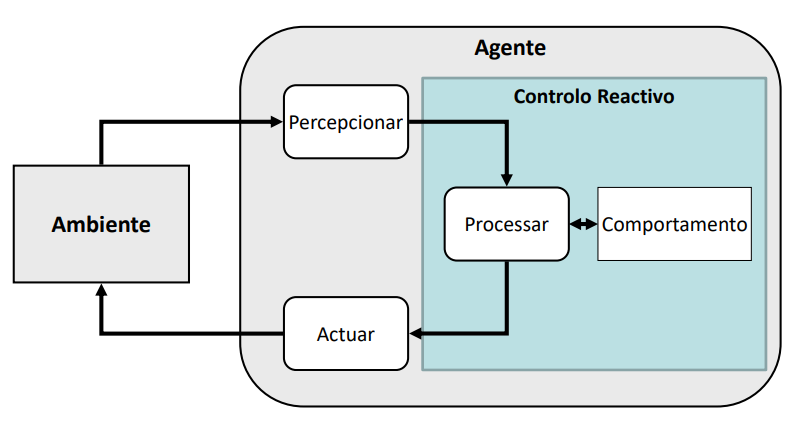
\includegraphics{../figures/controlo-reativo}}
    \end{center}
    \caption{Agente com controlo reativo.
    Retirado de~\cite{isel:iasa:slides:arq-agentes-reativos-parte-2}, slide 11.}\label{fig:controle-reativo}
\end{figure}


\section{Arquitetura Reativa com Memória}\label{sec:arquiteturas-reativa-memoria}

Numa arquitetura reativa com memória (ver figura~\ref{fig:arquitetura-reativa-memoria}), as reações dependem não só das perceções, mas também da memória de perceções anteriores (ou de informação delas derivada) para gerar as
ações. Para esse efeito é necessário manter internamente memória, a qual é atualizada a partir das
perceções e das reações ativadas, influenciando essas mesmas reações, bem como as ações
geradas~\cite{isel:iasa:slides:arq-agentes-reativos-parte-3}.

\begin{figure}[H]
    \begin{center}
        \resizebox{100mm}{!}{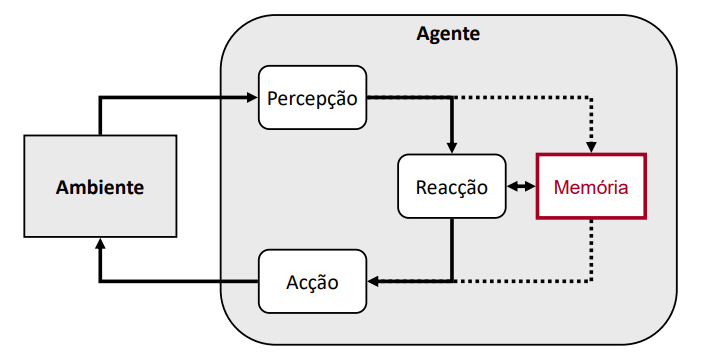
\includegraphics{../figures/arquitetura-reativa-memoria}}
    \end{center}
    \caption{Arquitetura reativa com memória.
    Retirado de~\cite{isel:iasa:slides:arq-agentes-reativos-parte-3}, slide 5.}\label{fig:arquitetura-reativa-memoria}
\end{figure}

O conceito de memória, associado a um comportamento, pode ser implementado de várias formas, como, por exemplo:

\begin{itemize}
    \item \textbf{Estado}: As perceções anteriores, que sejam relevantes, são armazenadas num estado interno do comportamento (ver figura~\ref{fig:agente-reativo-memoria-estado}), que é atualizado e consultado em função das perceções atuais e que influencia a geracão de ações (e.g., o agente move-se numa direção aleatória até que a contagem dos passos efetuados seja superior a um determinado valor, e só depois é que muda de comportamento);
    \item \textbf{Máquina de Estados}: Além de ter em conta as perceções atuais e as reações correspondentes, o comportamento pode ter em consideração entradas ou até um mecanismo de reset, que influenciam a próxima transição de estado e a consequente geração de ações e possíveis saídas (ver figura~\ref{fig:agente-reativo-memoria-maqest}).
    As entradas e saídas representam, neste contexto, interligações entre comportamentos~\cite{isel:iasa:slides:arq-agentes-reativos-parte-3}.
\end{itemize}

\begin{figure}[H]
    \begin{center}
        \resizebox{100mm}{!}{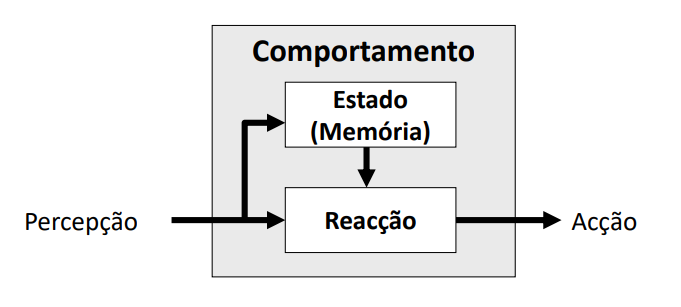
\includegraphics{../figures/agente-reativo-memoria-estado}}
    \end{center}
    \caption{Comportamento com estado.
    Retirado de~\cite{isel:iasa:slides:arq-agentes-reativos-parte-3}, slide 7.}\label{fig:agente-reativo-memoria-estado}
\end{figure}

\begin{figure}[H]
    \begin{center}
        \resizebox{100mm}{!}{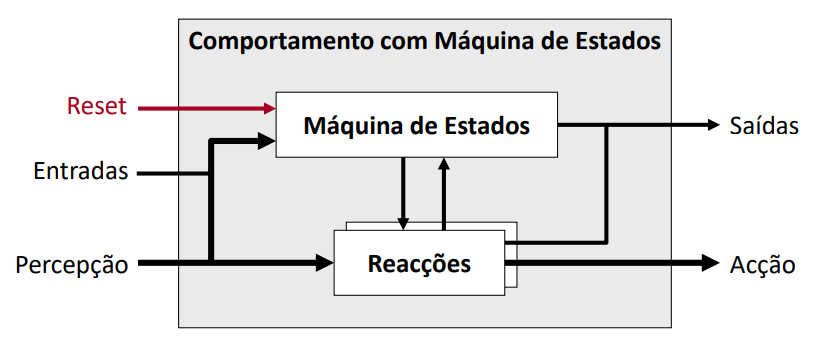
\includegraphics{../figures/agente-reativo-memoria-maqest}}
    \end{center}
    \caption{Comportamento com máquina de estados.
    Retirado de~\cite{isel:iasa:slides:arq-agentes-reativos-parte-3}, slide 8.}\label{fig:agente-reativo-memoria-maqest}
\end{figure}
\begin{table}[htbp]
    \centering
    \caption{Vantagens e desvantagens da manutenção de estado em arquiteturas reativas.
    Retirado de ~\cite{isel:iasa:slides:arq-agentes-reativos-parte-3}.}
    \label{tab:vantagens_desvantagens}
    \vspace{0.2cm}
    \begin{tabular}{|p{6cm}@{\hspace{0.8cm}}|p{6cm}@{\hspace{0.8cm}}|}
        \hline
        \textbf{Vantagens} & \textbf{Desvantagens} \\
        \hline
        \begin{itemize}
            \item Poder produzir todo o tipo de comportamentos;
            \item Representar a evolução temporal do comportamento do agente;
            \item Representar comportamentos complexos baseados na evolução temporal das perceções (e.g., agir devido à inexistência de um alvo após um determinado número de passos);
            \item Lidar com falhas, explorando novas ações (e.g., escolher uma nova direção após embater num obstáculo).
        \end{itemize}
        &
        \begin{itemize}
            \item Aumento da complexidade espacial;
            \item Aumento da complexidade computacional (i.e., manter as representações de estado);
            \item Limitações no suporte de representações complexas e exploração de planos alternativos de ação.
        \end{itemize} \\
        \hline
    \end{tabular}
\end{table}


\section{Biblioteca SAE}\label{sec:biblioteca-sae}

Para esta fase do projeto foi disponibilizada uma biblioteca em \textit{python} que apresenta e extende os conceitos expostos pela biblioteca realizada na primeira fase do projeto (ver capítulo~\ref{ch:projeto-parte1}).
Além disso, a biblioteca SAE (Simulador de Ambiente de Execução) permite a execução de um agente autónomo num ambiente simulado bidimensional, composto por alvos e obstáculos~\cite{isel:iasa:slides:sae-documentacao}.
Oferece, além de outras funcionalidades, a possibilidade de utilizar sete configurações de ambiente predefinidas.

A interface gráfica é composta por duas áreas de visualização (ver figura~\ref{fig:sae-interface-grafica}): a primeira área (à esquerda) apresenta a configuração do ambiente escolhida e com a indicação do agente; e a segunda área (à direita) é uma área de visualização de informação interna do agente.

\begin{figure}[H]
    \begin{center}
        \resizebox{100mm}{!}{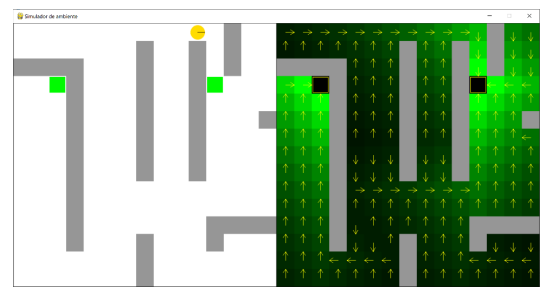
\includegraphics{../figures/sae-interface-grafica}}
    \end{center}
    \caption{Interface gráfica do SAE.
    Retirado de~\cite{isel:iasa:slides:sae-documentacao}, pág.
    3.}\label{fig:sae-interface-grafica}
\end{figure}

\section{Caracterização do Ambiente}\label{sec:caracterizacao-ambiente}

O ambiente onde o agente reativo se movimenta é virtual, bidimensional, com dimensões fixas e composto por alvos e obstáculos estáticos. Pode ser caracterizado (ver secção~\ref{sec:ambiente}) por ser:

\begin{itemize}
    \item \textbf{Totalmente observável}: O agente tem acesso a toda a informação do ambiente;
    \item \textbf{De agente único}: O ambiente contém apenas um agente a atuar;
    \item \textbf{Determinístico}: O próximo estado é unicamente determinado pelo estado atual e pela ação do agente;
    \item \textbf{Sequencial}: As ações do agente afetam as etapas consequentes (e.g., a recolha de um alvo implica a sua remoção do ambiente);
    \item \textbf{Estático}: O ambiente não muda enquanto o agente está a decidir a próxima ação a realizar;
    \item \textbf{Discreto}: O ambiente é composto por um número finito de estados possíveis.
\end{itemize}


\section{Implementação do Agente Reativo}\label{sec:implementacao-agente-reativo}

No âmbito desta fase do projeto, foram realizadas as seguintes tarefas:

\begin{boldenumerate}
    \item Definição de uma biblioteca denominada ECR (Esquemas Comportamentais Reativos) que expõe os mecanismos base de comportamento (ver secção~\ref{subsec:comportamento}), reação (ver secção~\ref{subsec:reacao}), estímulo, resposta, e comportamento composto (ver secção~\ref{subsec:comportamento-composto});
    \item Implementação de um conjunto de comportamentos e subcomportamentos que permitem ao agente autónomo atingir os objetivos propostos (i.e., recolher alvos e evitar obstáculos) utilizando a biblioteca ECR;
    \item Observação do comportamento do agente e da sua interação com o ambiente através da interface gráfica da biblioteca SAE;
    \item Adição de comportamentos mais complexos ao controlo do agente reativo de forma a melhorar o seu desempenho tendo em conta os objetivos propostos (e.g., inicialmente o agente apenas explorava numa direção aleatória, mas posteriormente foram adicionados comportamentos compostos de recolha de alvos e evitação de obstáculos); Ocorreu em simultâneo com o ponto \textbf{3}.
\end{boldenumerate}

Em relação ao ponto \textbf{2}, foram implementados os seguintes comportamentos:

\begin{itemize}
    \item \textbf{Recolher Alvo}: Representa um comportamento composto com um mecanismo de seleção de ação por hierarquia fixa de prioridade, que corresponde ao objetivo do agente prospector de recolher alvos.
    O agente deve, por esta ordem de prioridade, ter em consideração os seguintes subcomportamentos: (1) aproximar alvo; (2) evitar obstáculos; e (3) explorar o ambiente.
    \item \textbf{Aproximar Alvo}: Representa um comportamento composto com um mecanismo de seleção de ação por prioridade dinâmica, que corresponde ao objetivo do agente prospector de se aproximar de um alvo.
    Como a distância entre o agente e os diversos alvos varia consoante a posição do agente no ambiente (i.e., a intensidade do estímulo varia), o agente deve selecionar o alvo mais próximo (i.e., prioritizar o estímulo que apresenta maior intensidade) e por isso é que é usado um mecanismo de seleção por prioridade dinâmica (ver secção~\ref{subsec:comportamento-composto}).
    \item \textbf{Evitar Obstáculo}: Representa um comportamento composto com um mecanismo de seleção de ação por hierarquia fixa de prioridade, que corresponde ao objetivo do agente prospector de evitar obstáculos.
    É usado este mecanismo de seleção de ação, porque a próxima direção livre de obstáculos é calculada em função da posição do agente e dos obstáculos presentes à sua volta, de forma aleatória.
    E portanto, num dado momento, não existe uma direção livre mais prioritária (no sentido literal) que outra, mas sim, uma hierarquia onde estão definidas, pela ordem de descoberta aleatória, as direções livres de obstáculos encontradas.
    \item \textbf{Explorar}: Define um comportamento fixo sem memória (e.g., representação interna de perceções anteriores) e que, por isso está condenado à repetição. Está associado ao objetivo ``explorar'' e caracteriza-se por ter uma resposta fixa, pois gera uma ação em permanência, que consiste em mover-se numa direção aleatória. Não depende de nenhum estímulo para ser ativado.
\end{itemize}

Além dos comportamentos descritos, para os comportamentos compostos, foram implementados estímulos, respostas e reações, de forma a garantir a descrição e execução correta dos comportamentos associados.

Em paralelo ao desenvolvimento da implementação descrita e de forma a introduzir os conceitos de arquitetura reativa com memória, mais concretamente, o conceito de comportamento com estado (ver secção~\ref{sec:arquiteturas-reativa-memoria}), foi introduzido um comportamento que não caracteriza nenhum objetivo inicial descrito.
Este comportamento, denominado \textit{Contar Passos}, caracterizado por ser um comportamento fixo com memória, foi implementado com a finalidade de contar os passos do agente e tomar decisões com base no número de passos efetuados (e.g., ao fim de um determinado número de passos, o agente deve mudar de direção).
No entanto, tal comportamento não consta na implementação final do agente reativo, visto que não foi considerado relevante para a execução dos objetivos propostos.


\section{Estrutura do Projeto}\label{sec:estrutura-do-projeto-2}

No processo de desenvolvimento de software associado a esta fase do projeto, foi definida a seguinte estrutura em módulos e que está presente na pasta \textit{iasa\_agente/src}:

\begin{itemize}
    \item \textit{agente/agente\_reativo.py}: Integra a implementação do agente reativo;
    \item \textit{agente/controlo\_react}: Integra a implementação do controlo do agente reativo, bem como os componentes dos módulos comportamentais associados;
    \item \textit{lib/ecr}: Integra a implementação da biblioteca ECR;
    \item \textit{lib/sae}: Integra a implementação da biblioteca SAE, que foi disponibilizada para esta fase do projeto;
    \item ficheiro \textit{teste.py}: Executa o agente reativo implementado no ambiente simulado com a configuração escolhida, providenciado pela biblioteca SAE.
\end{itemize}
